\documentclass[11pt,a4paper]{article}

\usepackage{german,anysize,amsmath,amssymb,amsthm,paralist,array}
\usepackage{url}
\usepackage{graphicx}

\selectlanguage{german}

\pagestyle{empty}

\setlength{\textheight}{27cm}
\setlength{\parindent}{0cm}


\begin{document}
\textsc{Technische Universit"at Berlin}{\small\hfill 
Scalable Data Mining and Data Analysis}\\
{\small Database Systems and Information Management Group}

\bigskip
\centerline{\Large\textbf{Assignment}}
\centerline{\emph{Graph Mining with Stratosphere}}
\bigskip

\url{http://konect.uni-koblenz.de/networks/slashdot-zoo}

out.slashdot-zoo

de.tuberlin.dima.aim3.graphmining.Config#pathToSlashdotZoo

\textit{17 38 +1}


\centerline{\textbf{Network Statistics}}
\bigskip

\textit{de.tuberlin.dima.aim3.graphmining.statistics.OutDegreeDistribution}

\begin{enumerate}
\item \textbf{Determining the average ratio of friends and foes}

Schnubbidu

\vspace{5em}
\centerline{\textbf{Message Spread in Networks}}

lalala

		\begin{figure}[h]
			\begin{center}
				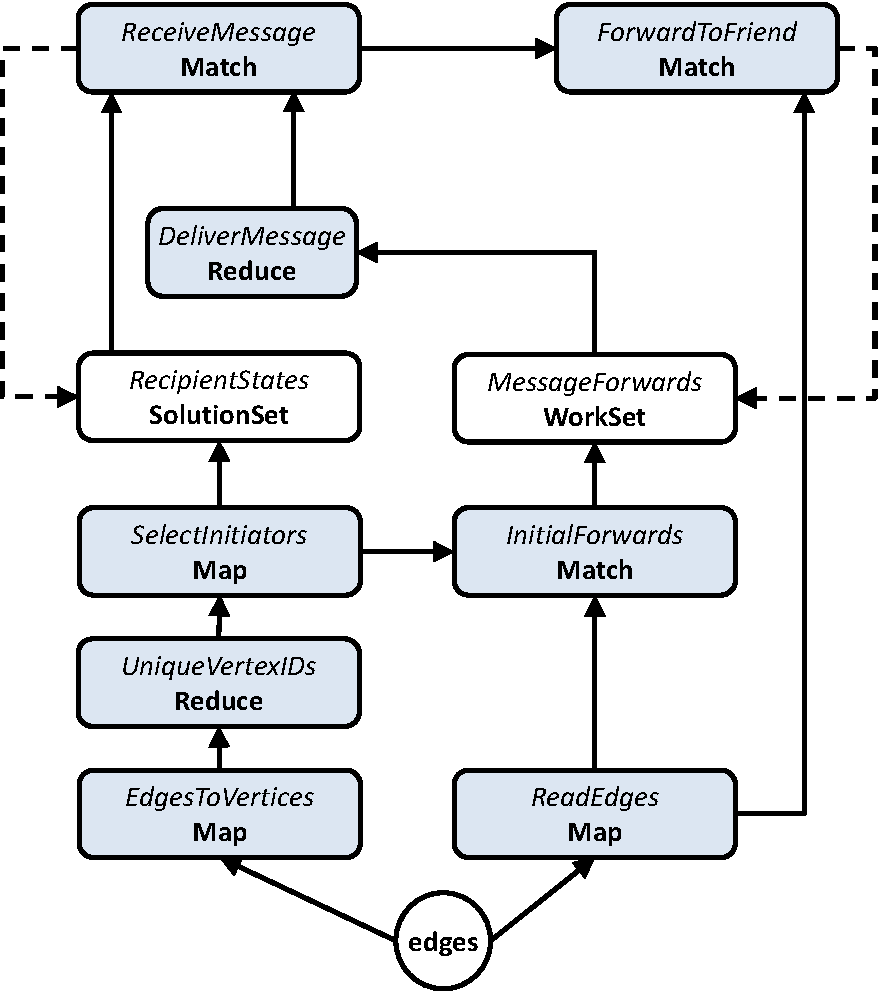
\includegraphics[scale=0.5]{chainletter-plan-crop.pdf}
			\end{center}
		\end{figure}


\item \textbf{Understanding the dataflow plan}

describe data flow plan

why is convergence guaranteed?

\item \textbf{Messages to friends only}

Modify the code to ensure that messages are only forwarded between friends.

\item \textbf{Increasing join performance}

modify plan to increase performance of initial forwards join 



\end{enumerate}

\end{document}
